#import "@local/bootlin:0.1.0": *

#import "@local/bootlin-yocto:0.1.0": *

#import "@local/bootlin-utils:0.1.0": *

#import "../../typst/local/themeBootlin.typ": *

#import "../../typst/local/common.typ": *

#show: bootlin-theme.with( aspect-ratio: "16-9", config-common(handout: "handout" in sys.inputs and sys.inputs.handout == "1", ))

#show raw.where(block: true): set block(fill: luma(240), inset: 1em, radius: 0.5em, width: 100\%)

#show raw.where(block: true): set text(size: 11pt)

#show raw.where(block: false): r => text(fill: color-link)[#r]

#show raw.where(lang: "c", block: true): set block(fill: luma(240), inset: 0.4em, radius: 0.5em, width: 95\%, breakable: true, above: 12pt, below: 12pt)

#show raw.where(lang: "c", block: true): set text(11pt)

#show raw.where(lang: "console", block: true):set block(fill: luma(240), inset: 0.4em, radius: 0.5em, width: 95\%, breakable: true, above: 6pt)

#show raw.where(lang:"console", block: true): set text(12pt)

 == Linux versioning scheme and development process

=== Linux versioning scheme
  \begin{itemize}
  \item Until 2003, there was a new ``stabilized'' release branch of Linux every
        2 or 3 years (2.0, 2.2, 2.4). Development branches took 2-3
        years to be merged (too slow!).
  \item Since 2003, there is a new official release of Linux about every
	10 weeks:
  \begin{itemize}
	\item Versions `2.6` (Dec. 2003) to `2.6.39` (May 2011)
	\item Versions `3.0` (Jul. 2011) to `3.19` (Feb. 2015)
	\item Versions `4.0` (Apr. 2015) to `4.20` (Dec. 2018)
	\item Versions `5.0` (Mar. 2019) to `5.19` (July 2022)
	\item Versions `6.0` (Oct. 2022) to `6.19` (Feb. 2026)
	\item Version `7.0` will be released in March/April 2026.
  \end{itemize}
  \item Features are added to the kernel in a progressive way. Since
        2003, kernel developers have managed to do so without having
        to introduce a massively incompatible development branch.
  \item For each release, there are bugfix and security updates called
    stable releases: 7.0.1, 7.0.2, etc.
  \end{itemize}


=== Linux development model
  Using merge and bug fixing windows
  \begin{center}
    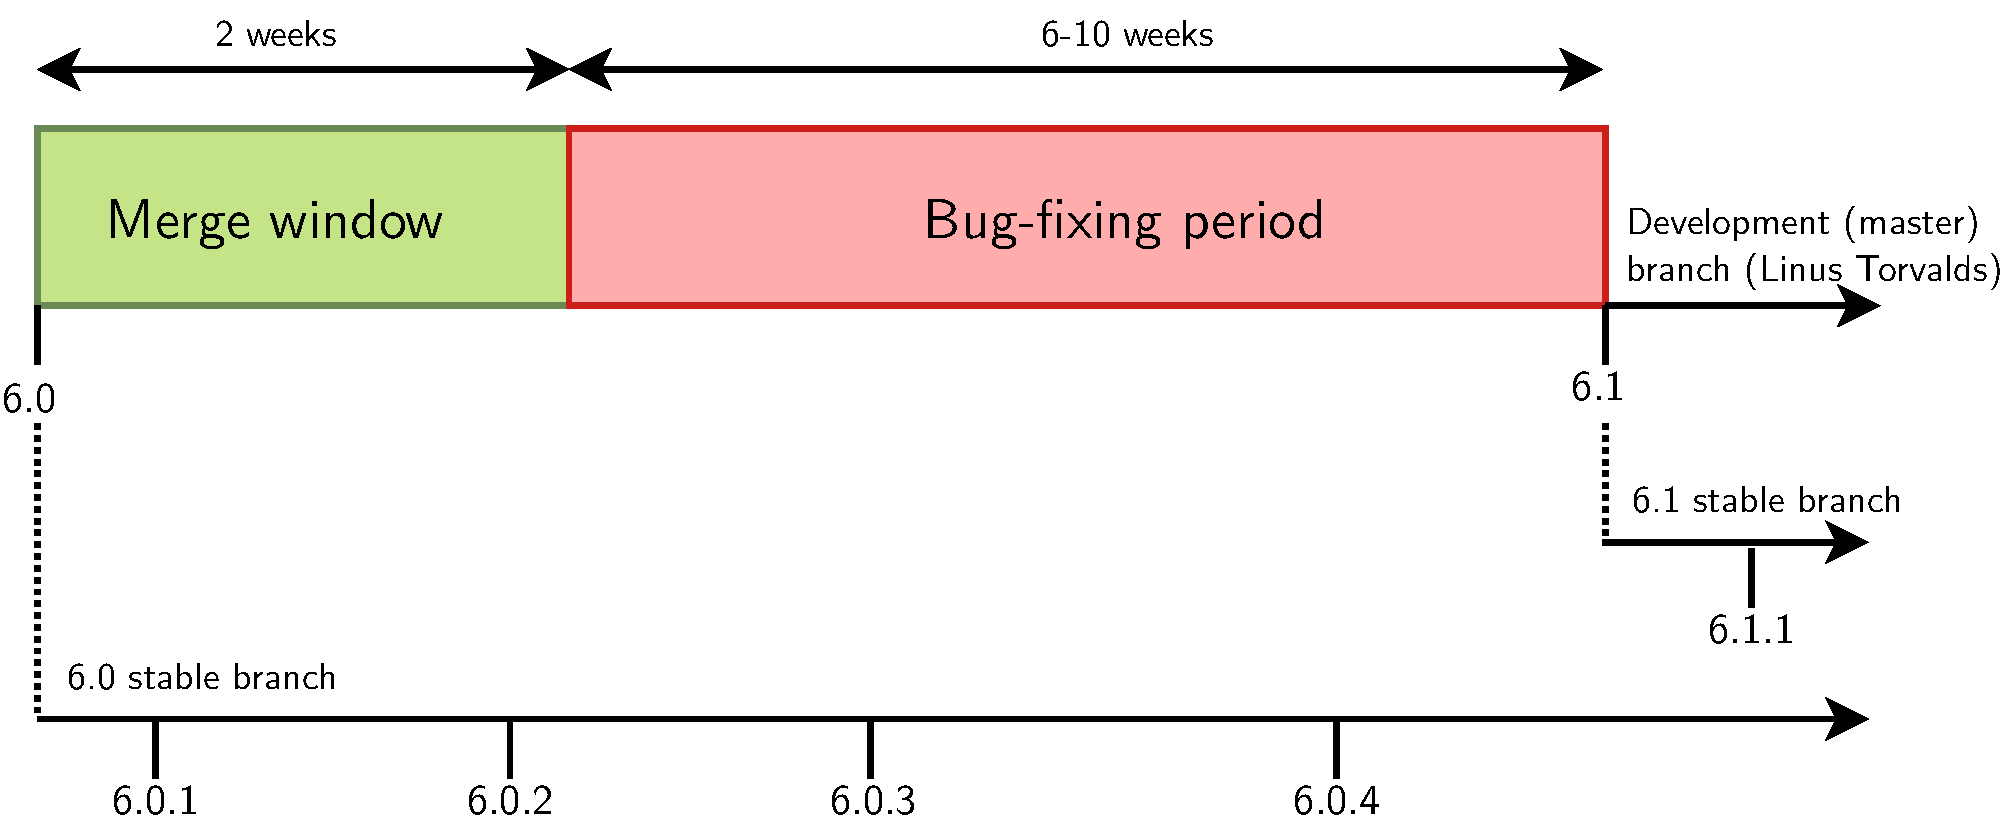
\includegraphics[width=\textwidth]{slides/sysdev-linux-intro-versioning/development-process.pdf}
  \end{center}


=== Need for long term support (1)
  \begin{itemize}
  \item Issue: bug and security fixes only released for most recent
    kernel versions.
  \item Solution: the last release of each year is made an LTS {\em (Long Term
     Support)} release, and is supposed to be supported (and receive bug
    and security fixes) for at least 2 years.
  
#table(columns: (50\%, 50\%), stroke: none,
[
  \includegraphics[width=\textwidth]{common/long-term-support-kernels.png}\\
  \column{0.4\textwidth}
  \scriptsize
   Captured on \url{https://kernel.org} in Feb. 2026, following the
   \href{https://www.kernel.org/category/releases.html}{\em Releases} link.
  \\]
  \item Example at Google: starting from {\em Android O (2017)}, all new Android devices
    have to run such an LTS kernel.
  \end{itemize}


=== Need for long term support (2)
  \begin{itemize}
  \item You could also get long term support from a commercial embedded
    Linux provider.
    \begin{itemize}
	\item Wind River Linux can be supported for up to 15 years.
	\item Ubuntu Core can be supported for up to 10 years.
    \end{itemize}
  \item {\em "If you are not using a supported distribution kernel, or a stable / longterm
    kernel, you have an insecure kernel"} - Greg KH, 2019\\
    Some vulnerabilities are fixed in stable without ever getting a CVE.
  \item The {\em Civil Infrastructure Platform} project is an industry /
    Linux Foundation effort to support much longer (at least 10 years)
    selected LTS versions (currently 4.4, 4.19, 5.10 and 6.1) on selected architectures.
    See \url{https://wiki.linuxfoundation.org/civilinfrastructureplatform/start}.
  \end{itemize}

